% !TEX root = ../main.tex
\chapter{Yuadrem} \label{ch::yuadrem}

\DndDropCapLine{B}{efore all other races, the tall kin}
stood, and created both conscience and sentience.
Also known as ets, the tall ones are a species with a history so old that their origin is muddied in rumors and myth.
While their intentions were mysterious, it is believed that they created the first kins.

Ets were obsessed with the preservation of the self and of their species.
They cured all ailments from illness and age, and we capable of molding their own flesh.
While the tall kin are long gone now, remains of their stone dwellings can be found all around Yuadrem.
Even above the wall of ice and stone and below the canopies of the elderberry wilds, their ruins stand strong and immutable.

Either by accident or conscious decision, the ets created the first four kins: the hardy gats, the mobile irds, the wise oths, and the playful marsets.
Ever haunted by the fear of death, the tall kin assigned each race a different task.
To search for the Lung of Ur, a relic of great importance to the ets.

Gats were created with the shape of goats by the indigo school of thought of Thul-yharch.
Adaptable and hardy, they were tasked with digging and searching the deepest caverns and ravines.

A product of the red school of Zyl'rech, irds were made in the image of birds.
They soared the skies along with their creators, surveying land and ocean with unparalleled efficiency.

The gold school of Tosh Drieln produced the arboreal marsets in the image of marmosets.
Their duty was to explore the deep reaches of forest and jungle, where the foliage was too dense to be seen from the high skies.

% Tol, yua'kch szua-tlekeloo
Finally, the oths were created by the enigmatic Tol, a schoolless et that disappeared long before the rest of its kin.
Educated and ingenious, they worked day and night recording and strategizing.
They coordinated the efforts of their siblings, making sure that no region was explored twice.

Either by design or by accident, all these newborn kins were unable to retain their sentience by themselves.
This ability was only conserved via a special token: the qualar.
Qualars are small totems made from bone and a strange black liquid known as qual ichor, obsessively crafted by the tireless et Ctereth.

Anybody who doesn't keep a qualars in its possession will lose their sentience over the course of a few weeks.
If its unable to obtain a new one, the poor creature will eventually be reduced to a ``lost one'', a shell of their former self.
A lost one's mind is partially lost, as they lose their sentience.
They are perfectly capable of abstract thought and able to understand their surroundings.
They are, however, incapable of perceiving themselves as something separated from the environment, and forever roam with empty minds.

During their search, the roaming marsets discovered two new kins from the Drejeck rainforests, the naenks and tsaneks.
Born of mold and fungi, these two were surprisingly not created by the tall kin, but by a conscious tree, Tekatsae.

The ets' obsession grew as did the vigor of their search.
This eventually coalesced as the eruption of the spire, an age-defining event known as the Schism.
This catastrophe swiftly ended the life of the ets, bringing with it decades of darkness and winter.
This defines the year 0 After the Schism --- or 0 AS.
The event was followed by a 40 year famine.

However, the strength of the event also created the sizzling gate, which is a hole to an outside plane only known as the outer lands.
This gate brought forth horrid creatures known as the blueblood beasts.
These fiends are terrifying abominations that hunt fauna and kin alike.

But not all beings that came from the outer lands were terrible.
Three foreigner kins also arrived from the gate: the adventurous tortles, the ingenious umans, and the violent grungs.
Quickly dragged to a raging ash storm, these creatures were forced to find home in a torn world.
While they eventually managed to live among the locals, their connection to the outer lands brings them problems to this date.
They are hunted by blueblood beasts and dark scholars, both permanently seeking their outsider blood.

Four years after the Schism, the zaloth arrived.
The zaloth are creatures born from storm, given conscience in strange circumstances.
They instinctively gathered qualar from the burning Jan'krug, living in the ruins after the fires subsided.
Eventually, they descended into the lacerated lands of Yuadrem.

Decades later, the last of the et-created kins was discovered: the quies.
Obedient and vigorous, the quies acted as servants to carry out the few duties their masters couldn't do.

Strangely enough, both foreigner and orphan kins require qualar to retain their sentience.
Lost ones of every race can be found in Yuadrem.
This suggests that the objects are related to the nature of sentience itself, rather than being a restriction imposed by the tall kin.

% !TEX root = ../main.tex
\subsection*{Qualars} \label{ssec::qualars}
\addcontentsline{toc}{subsection}{Qualars \& The Tides}

\DndDropCapLine{I}{n Yuadrem, sentience is not an ability}
to grow spontaneously in a being, but is related to a certain object: a qualar.
Qualars, or rluthe qual'yiz in jantherlin, are small bone totems filled with a strange black liquid named qual ichor.
All the peoples of Yuadrem need to keep a qualar close to them, lest they lose their sentience, devolving into ``lost ones''.
Lost ones are incapable to perceive subjectively, losing their sense of self.

Most qualars are made by one of the only surviving ets, a gargantuan being named Lua'Zheshal Qual'yiz Cter-Rheth, or Ctereth.
With bones provided by cultists and its own blood as qual ichor, the tall one tirelessly crafts the totems.

In oldentimes, qualars were assumed to be a limitation created by the tall kin to enslave their children.
However, when it was learned that the spontaneous kins like naenks, tsaneks, and zaloths still needed qualar, the hypothesis had to be quickly discarded.
Further confusing matters are the foreigner kins, who only started needing qualar after arriving at Yuadrem.

The sudden need for a qualar led each of the foreigner kins into two groups.
The first, who raided Ctereth and gained their qualars through effort.
And the second, who quickly lost their sentience and devolved into beasts.

While none can match Ctereth's handiwork, a few master bone carvers can craft imitations that replicate a qualar's properties, provided they can obtain the qual ichor to fill the totems.
Still, merely due to the qualars' value, it is common for the brave to attempt to steal the objects from Ctereth, endeavor that most usually results in new additions to its bone pile.

% !TEX root = ../main.tex

% The elusive white tide isn't explained here. The white tide is inaction, and is associated with observing events rather than taking part on them.
% Neither is the green tide, which concerns animal impulses.

% \begin{center}
%     \includegraphics[width=0.46\textwidth]{01yuadrem/img/02tides.png}
% \end{center}

\subsection*{The Tides} \label{ssec::tides}
\DndDropCapLine{N}{o one can tell how old the tides are.}
Some speculate that they were created by the tall kin in their search for individuality.
Others claim that they are simply part of the nature of Yuadrem.
No evidence asserts either of these viewpoints.

The tides represent complicated concepts that aren't entirely definable by language, but maybe are best defined as currents of emotions.
They flow within each individual's mind, deeply connected to qualars and sentience.
There are even ways to influence the tides of others, but they were quickly forbidden after their discovery.

They are as inviolate as air, and only a few are capable of perceiving them.
Their discoverers, the Igneist school of thought, gave them symbolic colors based on how they correspond with emotional reactions:

\subparagraph{Blue Tide} Wisdom, enlightenment, and mysticism.
It is the tide of the ones whose goal is to expand the mind and the spirit.

\subparagraph{Red Tide} Passion, emotion, action, and zeal.
It is the tide of the ones whose goal is to live in the moment, to experience life to its fullest, or to follow their heart wherever it leads them.

\subparagraph{Silver Tide} Admiration of power and the seek of fame.
It is the tide of the ones who seek to influence the lives of others or who actively seek to be remembered.

\subparagraph{Indigo Tide} Justice, compromise, and the greater good.
It is the tide of the ones who view life's difficulties from a broad, global perspective rather than an individual one.

\subparagraph{Gold Tide} Charity, sacrifice, and empathy.
It is the tide of the ones whose primary goal is to help others, especially at a cost to themselves.

These five tides form the basis of how actions are perceived.
None of these concepts are as simple as ``good'' or ``evil''.
A silver-aligned creature might use their fame to help someone.
A gold-aligned being might help someone purely for their own benefit.

The tides are linked to action, not intention.
For instance, someone could be falsely compassionate, but they will still be in the sphere of the gold tide.
Someone could unconsciously give itself to its passions, and they will still be moving along the red tide.
While the tides are linked to all, only a few truly understand their significance.
Even fewer know how to manipulate them, and those who do are severely punished.

The phenomena of the tides was discovered long ago in Ignelli.
Its manipulation led to the devastating tidal sway in 247 AS, and has been banned ever since.
No one can however deny that they are not compelled by the mere concept of the tides, and they are commonly used to describe people and ideas, for better or for worse.

\newpage

% !TEX root = ../main.tex
\section{The Continent} \label{sec::continent}

\DndDropCapLine{A}{ landmass so vast it houses all}
sorts of climates and biomes, Yuadrem is a supercontinent of impressive variety.
Many creatures of many natures interact with one another in its grounds, creating complex and diverse ecosystems and cultures.

Before any creature lived on the planet, the continent rose from the deepest of waters and established itself as a land amidst four violent seas.
It later became the cradle of civilization.
No matter how much change its inhabitants suffer, Yuadrem continues to stand as a testimony of the resilience of the ground, impervious to the business of its dwellers.

To distinguish its territories, Yuadrem is commonly divided into six regions: The Northern Territories, the Three Deserts, the Whaler's Sea, the Beryl Sea, the Barbaric Territories, and the Wildlands.

% TODO. Update each section to use tikzpicture for picture placement.
% !TEX root = ../main.tex

\begin{table*}[b]%
    \begin{DndTable}[width=\linewidth]{X}
        \centering
        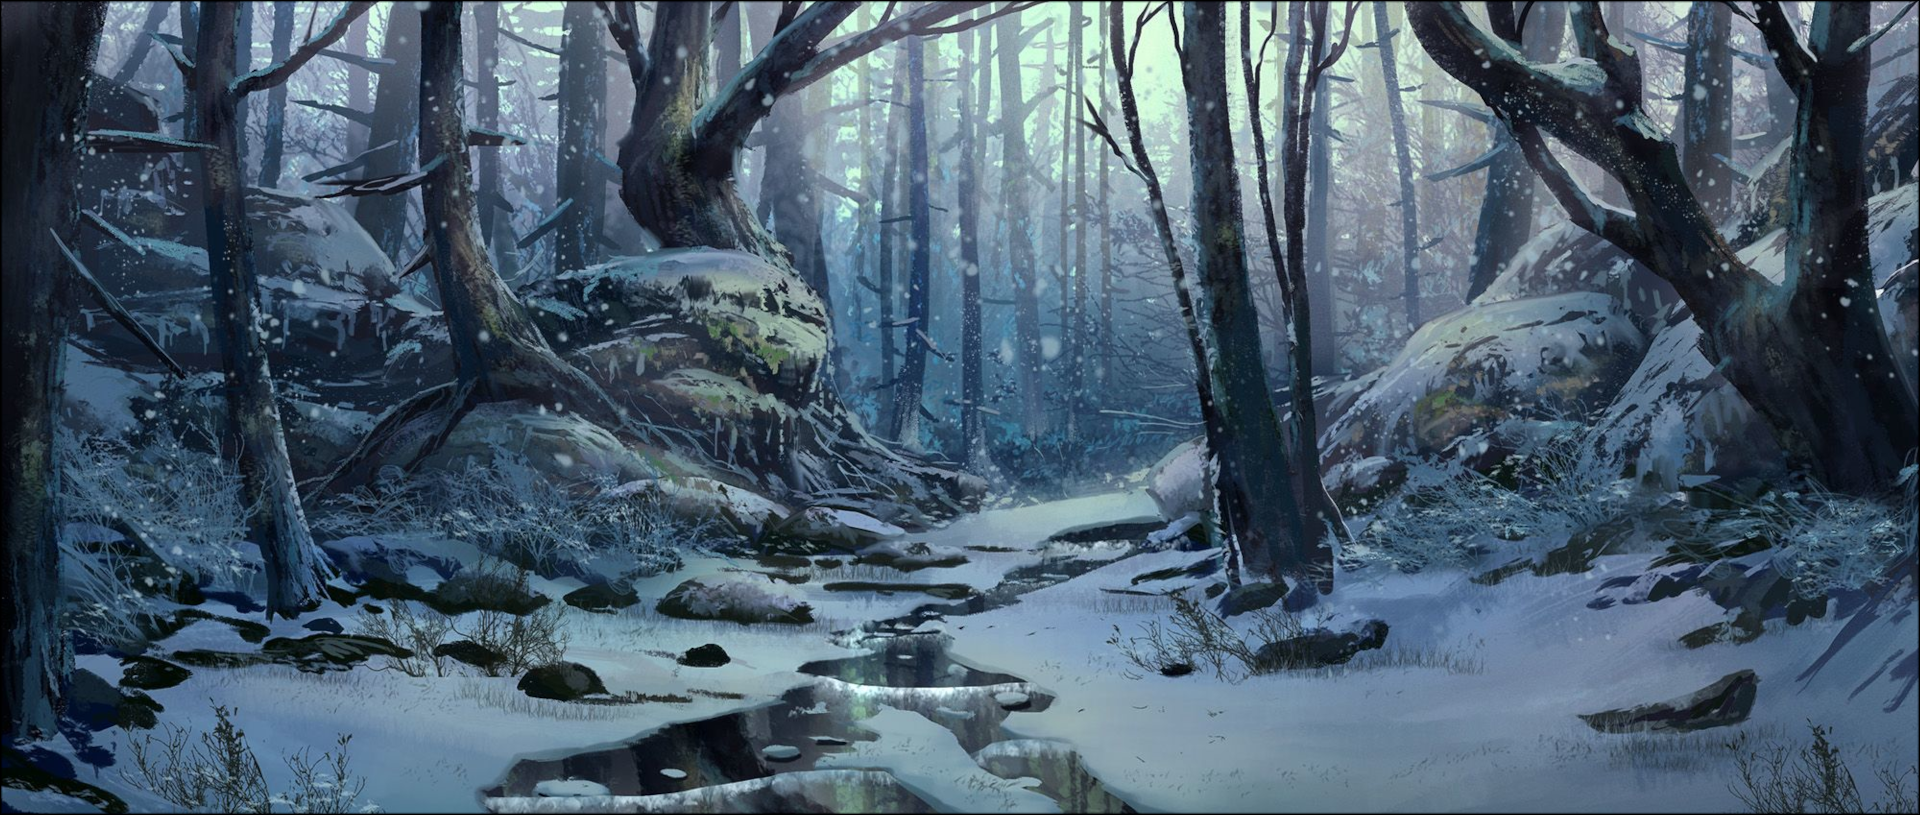
\includegraphics[width=0.95\textwidth]{01yuadrem/img/11tallwoods.png} \
        \centering \large{\textbf{The Tallwoods}}
    \end{DndTable}
\end{table*}

\subsection*{Northern Territories} \label{ssec::northernterritories}
The northmost region of Yuadrem, the Northern Territories are comprised by the Whitenorth, the Red Islands, the Tallwoods, the Blank Fields, and the Sulfur Lake.
The region is split by the Wall of Ice and Stone, a colossal mountain range that spans from coast to coast.

North of the wall is Whitenorth, an area split between the ancient ird kingdom of Krudzal and the territorial giants of Jatuunsa.
Its few inhabitants are beings of extreme resilience and fierceness, acclimated to the harsh habitat.
First among these are the giants, mountain-sized creature of stone, ever locked in war with Krudzal.

The middle of the region is characterized by the endless mists.
The area coincides with the north pole, and is inexplicably warm and misty despite its location.

To the west of Whitenorth is the Red Fjord, named so by its most common tree, the red maple.
The are is regarded sacred by the Krudzalians, who believe it to be the resting place of the sun god, Jua\~nanisz.
The fjord is currently occupied by Ribinhep, a uman nation ever standing up against the northerner irds.

Below the Wall of Ice and Stone are the Tallwoods and the Blank Fields.
The Tallwoods are an association of pine and redwood forest, using the mountains to hide from the cold winds.
The forests are devoid of civilized life, and the stone trolls who inhabit them make sure that they stay that way.

The Blank Fields are a vast, freezing tundra.
The low temperatures and strong winds in the area prohibit the growth of any vegetation.

The west of the fields are known as the Wurmlands, and they are solely inhabited by wurms.
Wurms are large reptile-like creatures that attack all foolish enough to approach their subterranean colonies.
The eastern portion of the land is filled to the brim with a variety of bughna gat tribes, ever in conflict for the large reserves of copper and coal in the mountains.

East to the fields is the Arctic Archipelago.
This cluster of islands separate the Whaler's Sea from the frigid ocean up north.
Mostly bare and desolate, the islets equally house ird, gat, uman, and zaloth settlements.

The strongest force in the archipelago is the Kaldrathal nation.
Having the only vessels strong enough to withstand the ship-sinking idzels, they regulate commerce in the entire archipelago.
% idzels or idzelal are inspired on Illhevi (https://abookofcreatures.com/category/iceland/page/2/).

% !TEX root = ../main.tex

% \begin{table*}[b]%
%     \begin{DndTable}[width=\linewidth]{X}
%         \centering
%         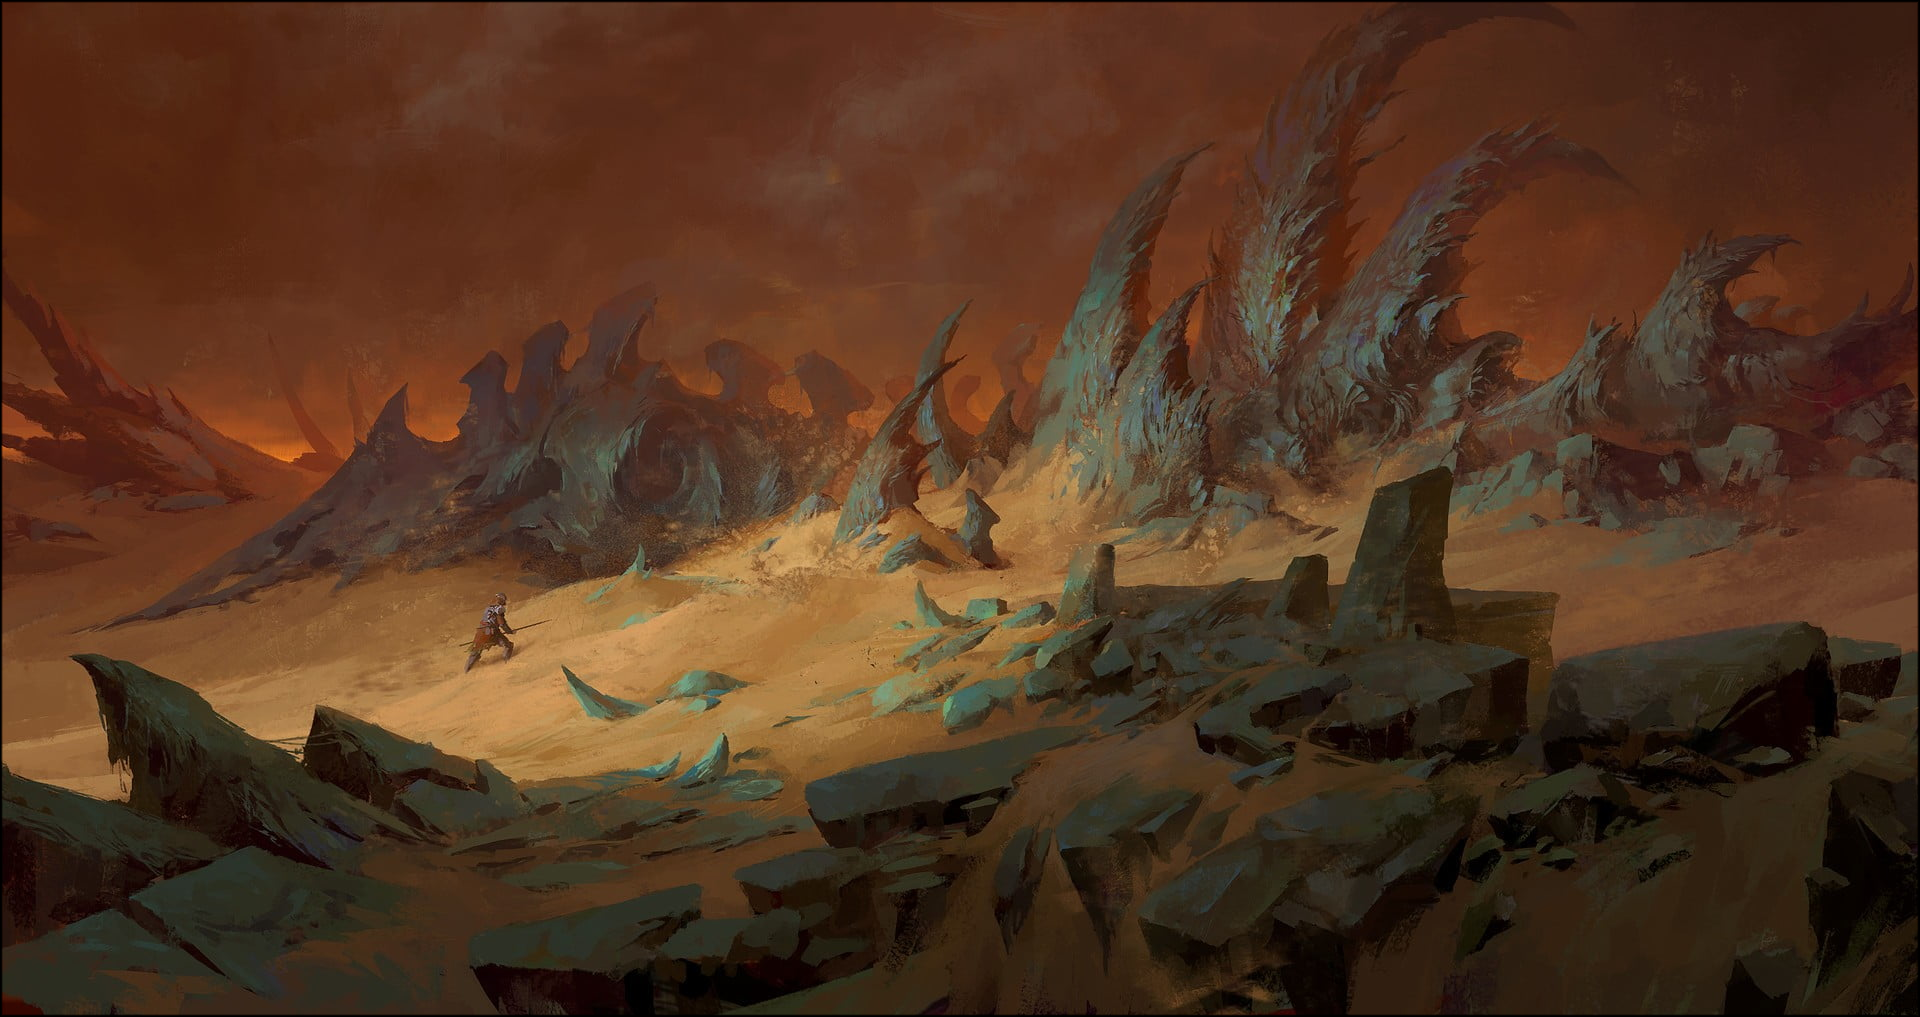
\includegraphics[width=0.95\textwidth]{01yuadrem/img/12dead_sea.png} \
%         \centering \large{\textbf{The Bone Cliffs of the Dead Sea}}
%     \end{DndTable}
% \end{table*}

\subsection*{The Three Deserts} \label{ssec::threedeserts}
Effectively splitting Yuadrem in half are the three deserts: Zoedrem, Zashlath, and the Dead Sea.

Zoedrem is a large expanse of yellow sands the embraces the waves of both the Whaler's Sea and the Teal Ocean.
The desert runs undisturbed from the Sulfur Lake down to the Defiled River.
It is commonly regarded as the most forgiving of the three deserts.

More fearsome than the sands are its inhabitants, the five dratl ird houses of Zoedrem.
Descendants of the fallen empire of Hulnar, they hide their settlements along the stone cliffs.
They are constantly in search of prey, robbing and murdering any traveler foolish enough to travel in their territories.

At the easternmost point of Zoedrem is the Sylvan Canyon, the only area in the desert able to host life.
The gorge is the home of the independent nation of Viphoger.
Apart from its inhabitants, the canyon's soil has rich natural deposits of oil, salt, and gemstones.
These resources grant Viphoger a strong economy despite its young age.

Southeast of Zoedrem and across the Ichor Mountains lie the Dead Sea, an artificial desert created by the tall kin's folly.
The desert's sands are of a sickly gray color, and any creature that inhabit the land for too long suffer particular mutations.
Its inhabitants, the treb gats and the cursed umans are perhaps the best examples of this.

The sands become blacker the more you approach the spire, the largest mountain in Yuadrem.
The et city of Jan'krug stands atop it, where the ritual that caused the Schism took place.
A long chasm divides the eastern region of the Dead Sea, remnants of the passage of the breathing island, Cabb Goem-Rlamesh.
Surrounded by hill, mountain, and river, the desert naturally prohibits passage to it, almost as if it's protecting a twisted secret.

Apart from the kins that call this desert home, the Dead Sea is infested with other monstrosities.
These are categorized into two: The Nyxborn and the children of Cabb.
The former are giant insect-like creatures that can be as large as an elephant and as precise as a mosquito.
The latter are tormented amalgamates that dislodged from Cabb Goem-Rlamesh, ever haunted by insatiable hunger and unending pain.

% Along with the tortles, grungs, and umans, the Schism brought forth terrible creatures known as the Nyxborn.
% These insect-like monstrosities can be as huge as the Mirmekolon, a colossal ant-lion hybrid, or as precise as the Khanokoladtes, a palm-sized moth that pierces skulls with its sharp dart-like mouth.

South, through the Hammerfall canyon, is the Zashlath desert, the driest of the three.
Featureless and white, only the hardy sunstruck oths have been able to call the desert home, and even they are wise enough to only establish by the neighboring mountains.

Zashlath practically receives no precipitation, and its white-colored sands reflect the scorching sunlight to deadly effect.
Truth is the desert remains largely unexplored to this date, and only rumors exist about the horrors that might hide among its sands.
Famous among these is the Haimorrois, a red horned snake whose bite forces the blood out of one's body.

% !TEX root = ../main.tex

\begin{figure}[t]
    \centering
    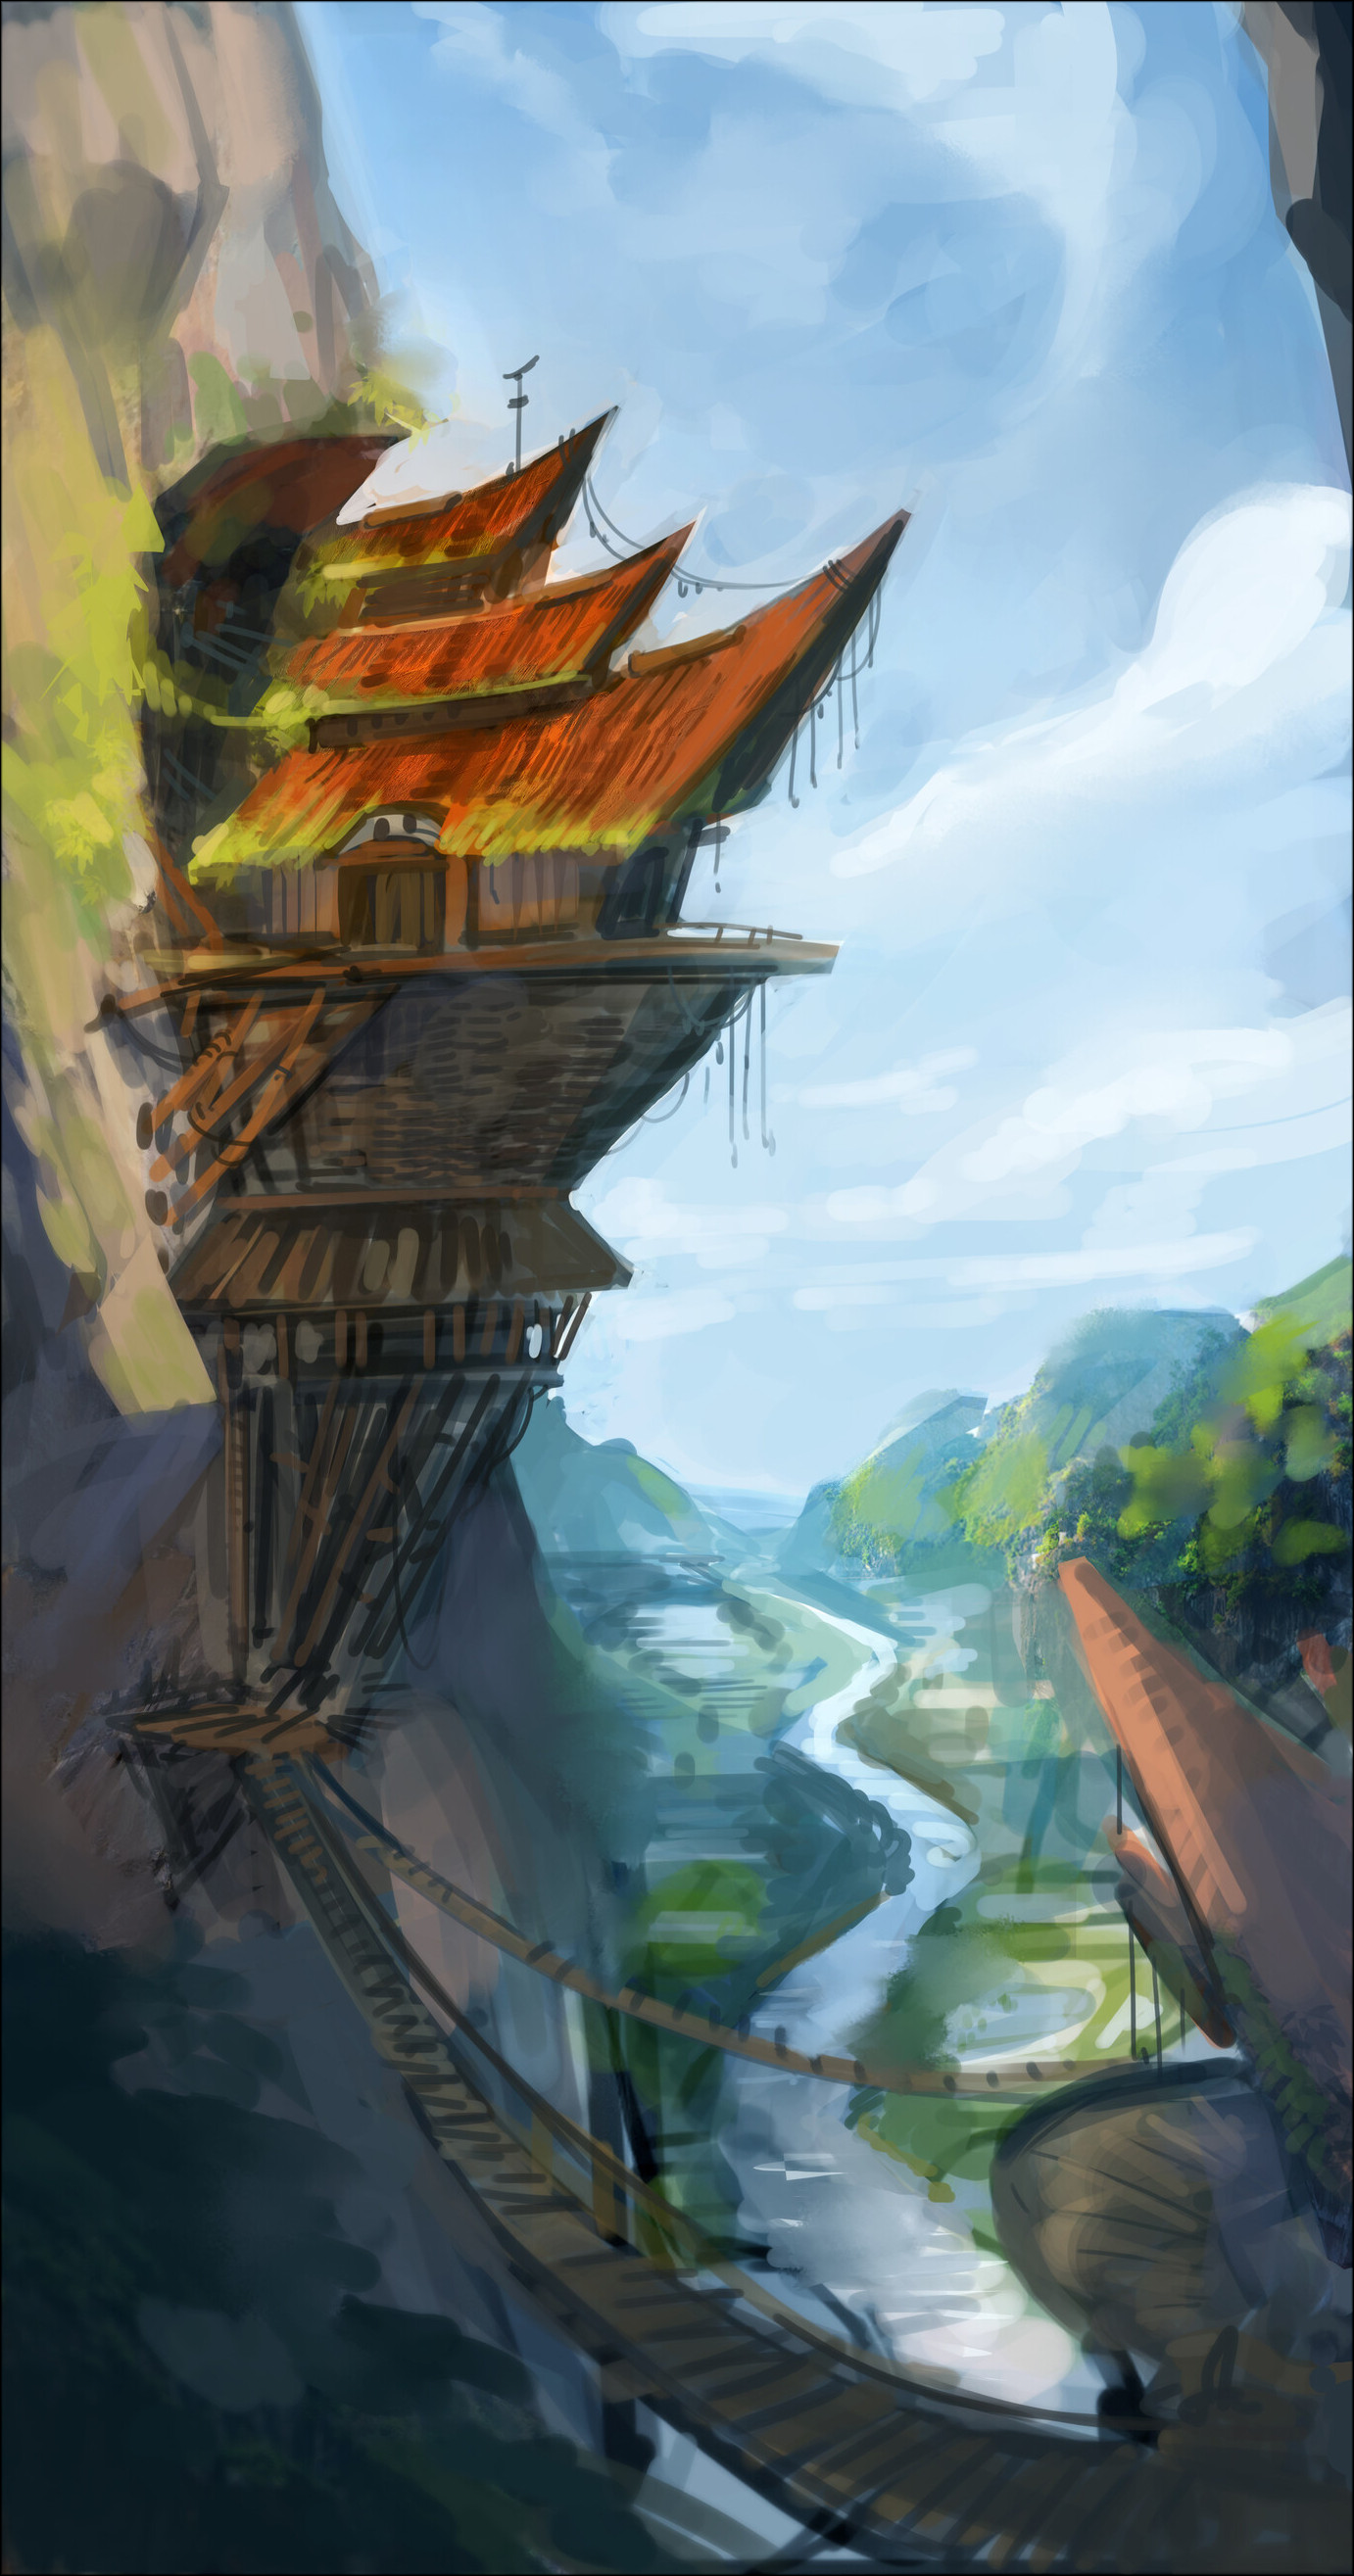
\includegraphics[width=0.46\textwidth]{01yuadrem/img/13siszgoel.png}
    \caption*{\centering \large{\textbf{Siszgoel, Kaldrathal's Capital}}} % TODO: Check if I can change the font of the caption
\end{figure}

\subsection*{Whaler's Sea} \label{ssec::whalerssea}

% intro
The cradle of modern civilization, the Whaler's Sea is home to both well-established and blooming countries.
Its coasts protected from harsh winds by mountain ranges and its cold waters supplied with both whale and idzel, the region couldn't be a better location to develop the modern world.
Idzels are large whale-like creatures known for their ship-sinking fury and their large supply of the valuable ambergris, the main ingredient in artificial qualars.

% Krejek and Kaljek
Sitting at the middle of the sea are the two southernmost islands of the Arctic Archipelago, Krejek and Kaljek.
The first is a large island covered by mountains, rocks plains, and deciduous forests.
It serves as the mainland for the independent nation of Kaldrathal.
%, who competes with Sulia as the main exporter of nitrate.

Starting out as a Krudzalian colony, they merged the quench-hardened steel of the thulkraka irds with their natural supply of nitrate.
This combination produces resilient steel firearms, including cannons, muskets, and flintlock handguns.
They remain the only exporter of these valuable weapons.

Kaljek, the smaller of the two islands, is a desolate land, with only few pine and birch forests.
It is separated by four nations inhabited by gat and ird alike.
While historically peaceful towards each other, they have recently been divided by conflict, all over the recently discovered gold veins that hide under their land.
% 661 AS: gold veins found under the ground.

% southern coast
South of both islands are the Horned Shores and the Fesh Peninsula.
The first is known for its calm, dry mediterranean climate, its sparse forests, and the great concrete gat city-states that rise from its ground.
Most of the land is devoid of natural resources, with scarce mines and low-quality wood.

% eastern coasts
East to these lands is the Fesh peninsula, an area inhabited mainly by gats, tortles and thulkraka irds.
A humid subtropical climate permeates the cape, and it is known for its harsh, capricious waters and frequent storms.
Also well-known are the tortles inhabiting the small island of Mbeat, for it is the only place where they have met safety after their arrival in Yuadrem.

In both regions lie the oldest nations of Yuadrem, the Seven kingdoms of the Sea.
Historically renowned raiders and pillagers, they are now famous for their passivity --- focusing on enterprise and artisanship.
What they offer is their expert craftgatship, and among them are the only bonecarvers capable of manufacturing qualars.

% western coast
Finally, to the west of Krejek one can find the two daughters of Palegna, the countries of Sulia and Drer.
The two nations were in a sense ``commisioned'' by the oth nation of Palegna.
Sulia was born to control the worrying growth of the Sulfur Lake, and Drer to restrict the growth of the bughna gat tribes of the Blank Fields.
% Both countries also served as an experiment of sorts for the word-obsessed oths, since the official language in both nations is the artificial Standard Language created by them.

Sulia benefited greatly from what would originally be their burden, and have developed a refined industry based on sulfur.
Their sulfur-based fertilizer is the basis of modern agriculture, their fiery blackpowder is only matched by Kaldrathal's, and their self-preserving wines are a taste craved all around the continent.
% They also have great sulfur-inlaid furniture!

Drer, in stark contrast with its sister, is a nation whose economy solely depends on pillage.
Re-imagining Sulia's blackpowder, they use their fire-bearing weapons to push back and raid their northern neighbors.

% !TEX root = ../main.tex
\subsection*{Beryl Sea} \label{ssec::berylsea}

The Beryl Sea is a searing, tropical region, ever battered by violent winds and waters.
The region is tapered in rainforests, and it houses two of the largest nations in Yuadrem: the warring Jenkashian empire and the mysterious Gannag.
The coasts see few other countries, and seldom do ships sail in these lands.
% Apart from the two, the coasts are also inhabited by a somewhat limited variety of countries, including the ancient Edede, the resilient Voskferm, and the strange Na'ane.

% Drejeck
Westernmost of Yuadrem is the thick, dark, and moist jungle of Drejeck.
Drejeck is the birthplace of the savage naenks and the ceremonial tsaneks, and is now entirely occupied by their nation, Gannag.
Despite being born even before the Schism, the beings of Gannag are primitive and untamed, and keep their tribal ways despite regular contact with more sophisticated cultures.
The jungle is also inhabited by large and dangerous beasts that threaten the unprepared explorer, like the aggressive nadubis or the silent whowie.
% And the bulettes and the Yara-ma-yha-who.

% Fog Gorge
East to Drejeck is the Fog Gorge, a well-forested canyon island ever enveloped in fog.
While primitive, the tribes of Gannag are far from free-living, and are bound by strong shackles to their superiors.
While naenks are used to this hierarchical system, many of the more intelligent tsaneks grow tired of it over time.
A hundred and fifty years ago, a group of tsaneks went as far as to establish their own independent tribe of Na'ane in the misty island, abandoning their brethren in favor of an unrestrained lifestyle.
Freely they carry on with their ceremonies and rituals, protected from their neighbors by mist and stone.

% Qul archipelago
Further east one finds the Qul archipelago, a clump of islands that collectively served as the birth bed of the Jenkashian empire.
Jenkash is a coalition of tribes that only managed to unite after cutting down the last tree in their mountainous islands.
This led to an explosive expansion of their empire, and they swiftly conquered the neighboring lands.
Their territories now span most of the coasts of the Beryl Sea.

The archipelago itself is absolutely desolate, with barely any tree or foliage growing atop its igneous rock.
Perhaps the only bright side of this uncontrolled deforestation is the fact that it brought to light the iron and diamond veins in the eastern side of the archipelago.
These resources are heavily exploited by the qulbaba irds, and led to their signature diamond daggers.

% Dratl'fal savanna
North of the archipelago is the Dratl'fal savanna, occupied entirely by Jenkash.
The only plant that freely grows in the savanna is bafarmat, a purple moss covering its entire southeastern coast.
This plant is the primary food source of the cavernous species that live under the ichor mountains.
Its spread has allowed the hornbeetles to move into the area, a strong species of giant blue beetles that served as companions to the now ruined nation of Phrisht.

In oldentimes, the dry lands served as the birth bed for many gat city-states, of which only Dzorvepem and Jorea remain standing, now part of Jenkash.
Despite its lack of resources, the whole area was sought after by the now divided empire of Hulnar, who battled against the blooming nation of Phrisht for more than 300 years for it.
This everlasting conflict was only stopped by Jenkash, who in their thirst for conquest ended up dissolving the untiring countries.

% \begin{figure}[t]
%     \centering
%     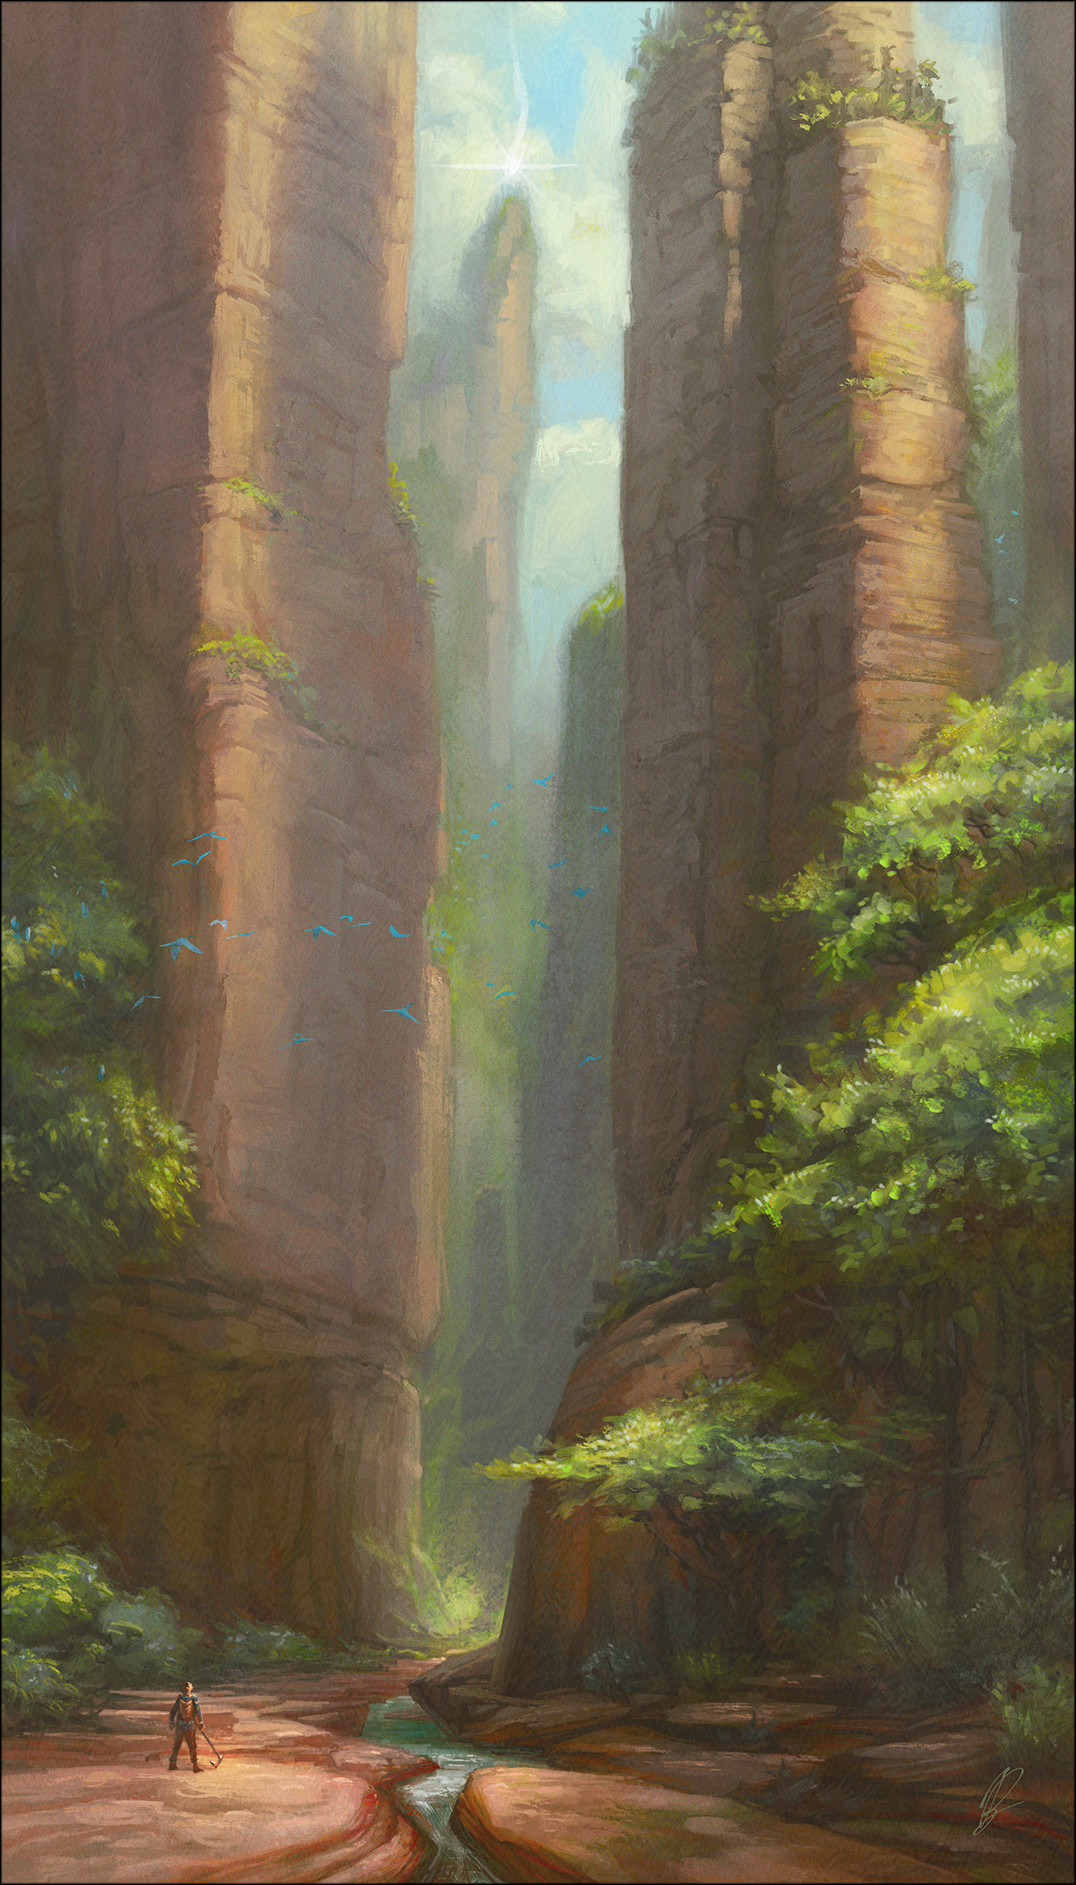
\includegraphics[width=0.46\textwidth]{01yuadrem/img/14fog_gorge.png}
%     \caption*{\centering \large{\textbf{The Fog Gorge}}}
% \end{figure}

% Ironlakes Island & Zashlath savanna
Moving to the easternmost portion of the sea one can find the Ironlakes Island and the Zashlath savanna.
The former is a large island full of forests and lakes.
It was historically a part of the peaceful marset nation of Edede, but most of it now belongs to the warring empire.
The Zashlath savanna is the area west of the desert, protected from its dry air by the moisture of the cerulean waters.

% !TEX root = ../main.tex

\begin{table*}[b]%
    \begin{DndTable}[width=\linewidth]{X}
        \centering
        \includegraphics[width=0.98\textwidth]{01yuadrem/img/15om.png} \
        \centering \large{\textbf{Om, Isken's Capital}}
    \end{DndTable}
\end{table*}

\subsection*{Barbaric Territories} \label{ssec::barbaricterritories}

To the east of Yuadrem are the Barbaric Territories, a region defined by the brutality of war and the greed of an empire.
From north to south, the land can be divided into five areas, each with its own distinct characteristics: the Drylands, Cabb Goem-Rlamesh, the Shield Sea, the Chirping Wilds, and the Xuam Peninsula.

% Drylands
Northernmost are the Drylands, a field devoid of trees or any sort of tall flora.
The area is plain and parched, dried over the years for its lack of rains or rivers.
The northernmost area of the savanna remains bare to date, and is the most tortuous stretch between the Fesh Peninsula and the southern nations.

% Mzavit river and southern savanna
Down across the Mzavit River, the savanna becomes humid and with this water comes civilization.
A wide array of gat city-states have been established here.
Able to withstand the thunderous force of the Jenkashian and Iskenese armies and the hulking chimeras from the Next, these states are noteworthy for their fortitude.
Of special note is the adamant country of Byurev, who have halted the growth of Isken for almost three centuries.

% Cabb Goem-Rlamesh
% NOTE: In the whole island of Cabb Goem-Rlamesh a faint crying sound can be heard.
Off the coast of the Drylands lies a place known as the breathing island, Cabb Goem-Rlamesh.
A harrowing immensity, the landmass is constructed entirely of flesh and bone, and is believed to be what remains of the ets.
Not much is known about the island, and none of the few explorers who have travelled to it retain their sanity.
The mad tell tales of a mortifying city of flesh, and of strange, shape-shifting inhabitants.

% Shield Sea & The Nest
% Wrong information - geomancy was invented by an ancient civilization that warred with the tall kin eons ago, but was erased from history by the victors. There are ruins from this civilization at the basin of the lake, and Fo is the last remaining member from it.
Southwest of the Drylands rest the Shield Sea, an enormous body of water fed by a wide array of tributaries from the Forking Peaks.
In antiquity, the ruined ird civilization of Hairuus invented the art of geomancy in its coasts, raising from the basin the island of ``The Nest'' at its center.
The island currently hosts only one being, Fo.
Fo is a strange creature, rumored to be out of this world.
It welcomes visitors with a variety of fierce chimeras.

% Chirping Wilds
Southeast from the Drylands and passing through the Do Nana swamp are the Chirping Wilds, a vast and largely untamed rainforest.
The jungle is inhabited only by the Iskenese empire, a large grung nation that expelled the original ird and marset population.
The only territories currently not held by the grungs' military might are the strong qulbaba irds of Harual to the west, and the marsets of Uzuz from the Xuam peninsula.

The Xuam Peninsula is the southermost point of the Barbaric Territories, and is located just south of the Grasping Gulf.
The region has facilitated the development of Uzuz due to the heavy presence of wurmroot, a white-leaf poplar tree that is conveniently toxic to all foreigner kins, specially to grungs.

% !TEX root = ../main.tex

% \begin{table*}[t]%
%     \begin{DndTable}[width=\linewidth]{X}
%         \centering
%         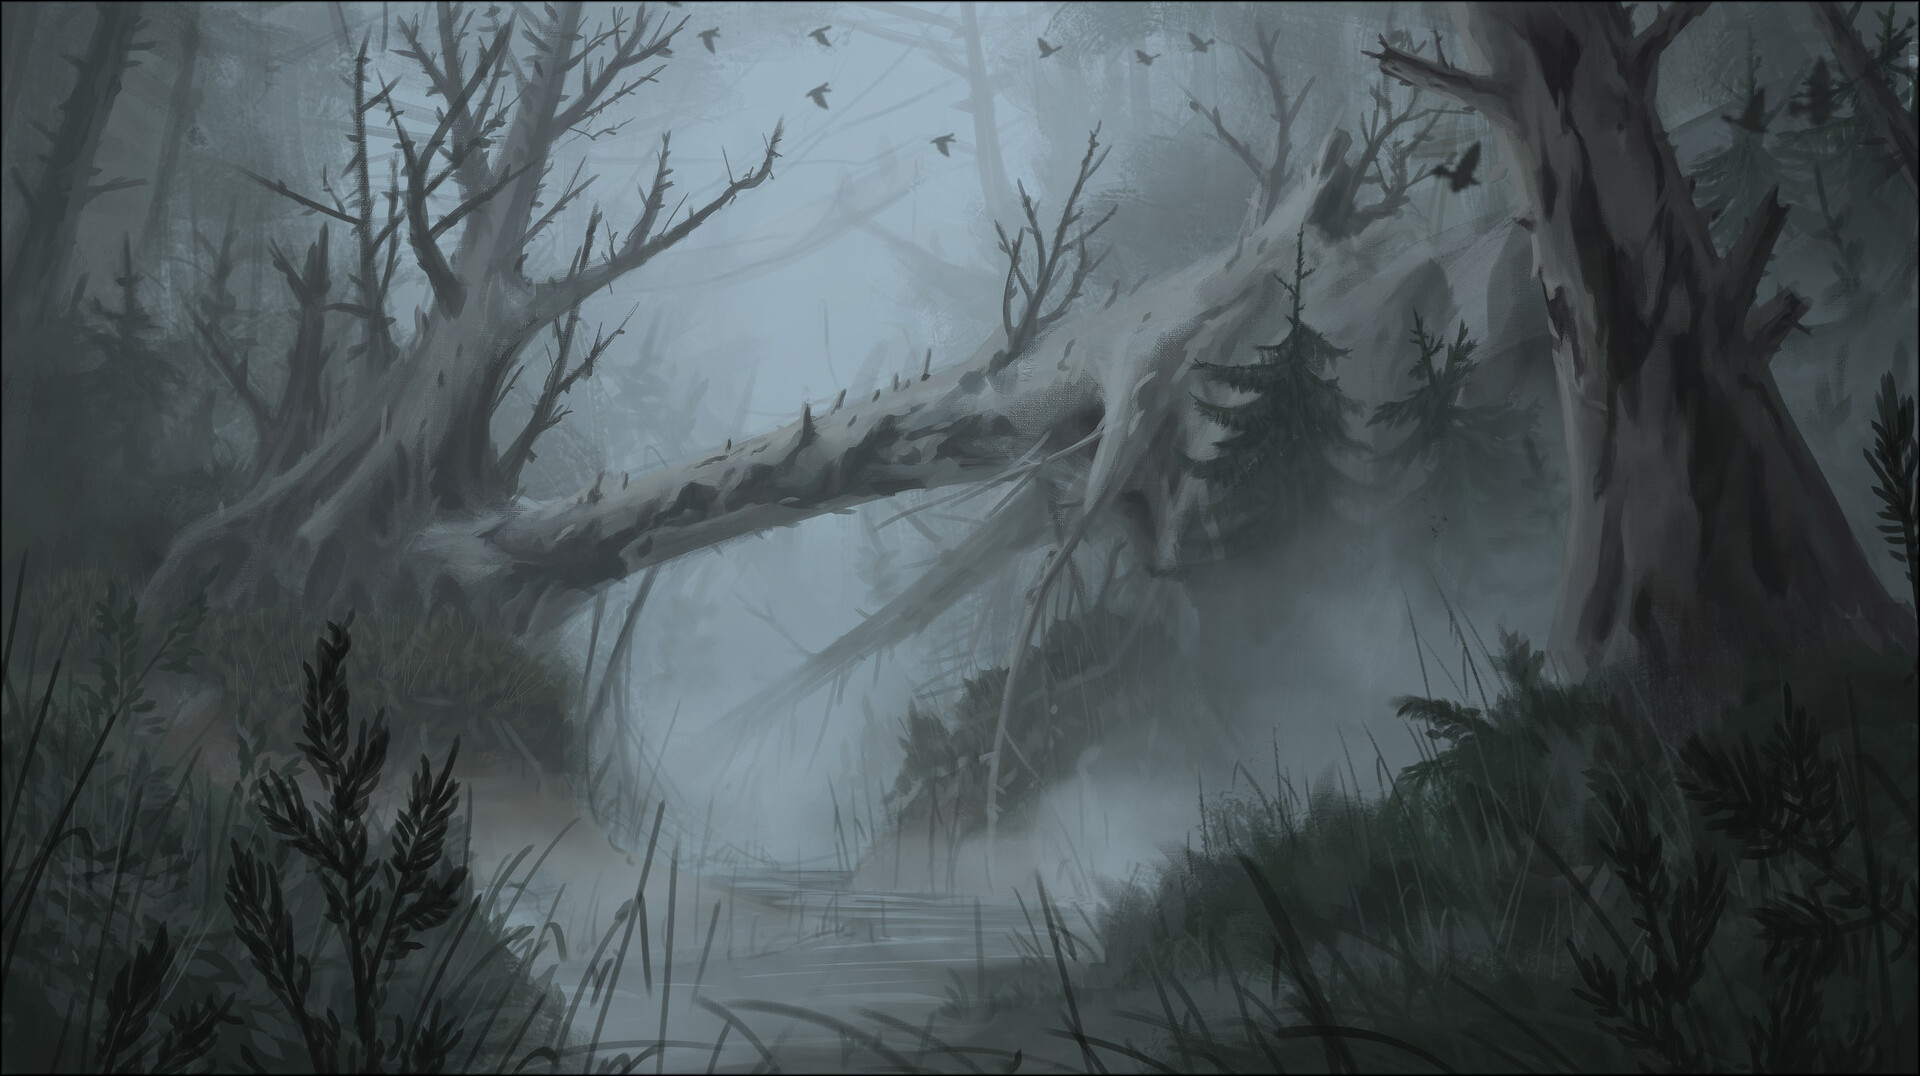
\includegraphics[width=0.98\textwidth]{01yuadrem/img/16pale_blemish.png} \
%         \centering \large{\textbf{Forests Surrounding the Pale Blemish}}
%     \end{DndTable}
% \end{table*}

\subsection*{Wildlands} \label{ssec::wildlands}

% intro
The southernmost region of Yuadrem is aptly named the Wildlands, for it is a large expanse of untamed fields, forests, and lakes.
Starting at the bottom-most part of the forking peaks, the area has seen very little intervention from the civilized world.
This is attributed to the fact that the Wildlands are infested with both deadly creatures and strange tide-altering illnesses.

% Savage Plains
Just below the forking peaks and the Beal river is the northmost point of the Wildlands, the Savage Plains.
They are a humid subtropical area covered by marshes and plains, with few patches of forest in-between.
Fed by many rivers from the mountains, the lands define the southern territories of the Iskenese empire, expanding thorough the whole region.

However, Isken's grip on the Savage Plains is tenuous at best, as the region is as much controlled by the grungs as it is by the local wildlife.
Just as in the forest below, a great variety of foul beasts and creatures can be found in these swamps.
Of special note among these are the giant mole-like jinshus, beasts unique to region who suffocate the unprepared by sinking them beneath the earth.

% Everwoods
As dangerous as these plains are the Everwoods, the forest that grows south of them.
This ancient woodland used to be a place of respite after the harsh swamps, but all that swiftly changed about 400 years ago.
In an attempt to manipulate the tides, the Rashiist school of thought from Ignelli summoned The Sorrow into Yuadrem.
The Sorrow is an entity of unknown origin, who seeped into Yuadrem due to the Rashiists folly.
On arrival, it swiftly slayed all members of the school of thought, and brought fourth with it strange creatures and diseases that now plague the once peaceful forest.
This event came to be known as the Tidal Sway.

% Pale Blemish
Not only bringing forth pain and disease, the Tidal Sway also ravaged the land around Ignelli, area now known as the pale blemish.
All flora was destroyed, and the ground turned into badlands.
The field now serves as a grim reminder to all of the dangers of manipulating the tides.

Despite the destruction, the scholars from the Igneist school continue to work in their temple, studying the tides and The Sorrow.
Perhaps one day they'll achieve their goal and undo their sister school's sins, expelling the Sorrow and healing their lands.

% Niknek Peninsula
West of the Everwoods is the Niknek peninsula, a thin, elongated stretch of land filled with volcanoes and gorges.
The cape was spared from most of the effects of the Tidal Sway.
Niknek and the nearby Vuvu Isles now house the refuge marsets from the Ironlakes Island.

% Elderberry Wilds
At the southern tip of Yuadrem are the Elderberry Wilds and the Ironwoods, a set of pine and spruce forest surrounding the Manta Sea.
The area is partly occupied by Gronselar, an old and forgotten colony of Krudzal.
% Not much is known about these forests due to their remote location.
% Not much is known about the area due to its remote location, but even here a semblance of civilization exists. in the form of the ird nation of Gronselar, and the regions of Froibias, Glameas, and Visilias.


% !TEX root = ../main.tex
\section{Cultures} \label{sec::cultures}

\DndDropCapLine{U}{pon their abandonment, the kins were}
quick to travel to the far reaches of Yuadrem, carrying civilization with them.
Over the years, languages, religions, and rites of different natures spreaded far and wide to create the complex network of cultures we see today.

% !TEX root = ../main.tex
\subsection*{Religions} \label{ssec::religions}

\DndDropCapLine{R}{eligion is an important part of life}
of the many cultures of Yuadrem.
Some worship specific pantheons of gods, others praise unpersonified concepts, and a selected few worship nature itself.
% In the times before the schism there was a wide belief that the tall kin could answer prayers, but their worship is now forbidden in most of the continent.

% The true existence of these divinities is a widely discussed subject, but their worship is undeniable.
From the nature-worshiping folk of Jenkash to the god-birds of Krudzal, each culture performs a set of rituals in the name of their deities, and some even claim to be able to channel their divine power.
While it might be hard to pinpoint the exact number of religions in Yuadrem, a few are built into the fabric of civilizations, and are easy to tell apart.

\subsubsection{Igneism}
The oth scholars hailing from Ignelli were the first to conceptualize the tides.
They learned that the tides are intrinsically woven into sentience.
As tightly tied threads between sentient creatures, a change in the tidal alignment in one has profound effects in that of those nearby.
% Each tide was then assosiated with a symbol and an entity, to give a more concrete face to it and facilitate its worship.

The blue tide is represented by a blue unfinished book, representing the eternal pursuit of knowledge.
The gold tide is symbolized as a seed or an egg, telling of the coming of future life with proper nourishment.
Indicated by a torch, the indigo tide tells of the truth revealed under light, and the punishment exerted upon those who hide it.
A broken compass represents the red tide, representing the roaming of those who walk without roads.
The silver tide's symbol is a bell, denoting the attention obtained by those who seek fame.

Nearing the year 174 AS, the knowledge of the tides split the Ignelli school in two - The Igneists and the Rashiists.
% The Zelseists, who simply sought to further understand this new discovery, and the Rashiists, who attempted to wield and manipulate them.
The latter created a system of magic known as Rashid, with which they could potentiate the tidal alignment of others.
Despite the warnings issued by their sister school, the Rashiists honed their craft to its maximal potency, and suffered severely from it.
Their actions awoke a strange an antique and mysterious creature: The Sorrow.

% The Sorrow is a being of indescribable shape who was summoned to Yuadrem by the Rashiists' folly.
Breaking the mind of any who lay their eyes upon it, it swiftly took the lives of all who corrupted the balance of the tides, thus ending the Rashiist school's folly.
Its presence caused the pale blemish, and with it came horrid creatures known now as the xuagra.
Seeing the destruction caused by their sister school, the Igenists hid the knowledge of their former brethren, forbidding Rashid in any shape or form.
% Finally, they changed their own name to Igneists in an attempt to bury the other school in anonymity.

Igneism is the worship of the tides as a concept, and the active pursuit of keeping the five balanced.
Igneists recognize that sentience cannot exist without the tides, and praise them as thanks for the capacity of independent thought.

\subsubsection{Tanethism}
Across the long history of the Seven Kingdoms, varied deities were gradually associated with many different concepts, and any gat would pray to different gods at different times and circumstances.
For example, one might say a prayer to the Traveler for luck, make an offering to Tamaz before going to the market, and pray to appease Matevos when a severe storm blows in --- all in the same day.

Independent to any institution, the gat scholar Taneth officially published ``The Rituals and Gods of the Gats'' in 511 AS.
The book was an exhaustive compilation of the more than a thousand deities that were praised by the different kins of the Seven Kingdoms, and proposed a reduced pantheon of 15, distilling the chaotic pantheon into the main gods.
Taneth's work was barely known during their life, and they died without due recognition.

Later, in the year 577 AS, the king of Khedrat Olag the Immortal sought a method to reduce the religious disparity among their people.
Either by divine will or happenstance, they came upon this book by Taneth, and established Tanethism as the official religion of Khedrat, imitating the well-established creed of other nations.
By command of the government, many churches were erected in the name of each god, and the many gods of the gats coalesced into a more sober pantheon of 15.

Many have a favorite among the gods, one whose ideals and teaching they make their own.
A few even dedicate entirely to a single deity, serving as a priest, acolyte, or champion of that god's image.
Famous among these devout beings are the nimrod, an organization of zealous hunters of Phusinhe who pursue all who disturb the balance of Yuadrem.
Well-known as well are the followers of Havetish, a group of gats in golden robes whose goal is to distribute wealth and food to the impoverished hamlets of the inner regions of the Seven Kingdoms.

\begin{table*}[b]%
    \begin{DndTable}[width=\linewidth, header=The Gods of Yuadrem]{p{2cm}p{0.8cm}p{3cm}p{1.8cm}X}
        \textbf{Name} & \textbf{Tides} & \textbf{Domains} & \textbf{Religion} & \textbf{Symbol} \\
        The Scholar  & B  & Reason, Knowledge     & Igneism   & A many-armed blue oth reading multiple books. \\
        The Zealous  & R  & Passion, Zeal         & Igneism   & A red dratl ird standing over a sand dune. \\
        The Star     & S  & Admiration, Fame      & Igneism   & A naked tall one, sometimes replaced by a shadow or a uman. \\
        The Equalist & I  & Justice, Equity       & Igneism   & An indigo gat holding a spear and a coin. \\
        The Altruist & G  & Empathy, Compassion   & Igneism   & A furtive golden marset carrying a basket full of eggs. \\
        The Sorrow   & -  & Balance, Punishment   & Igneism   & An indistinct cloaked figure holding a bloody heart. \\
        Changing God & -  & Secrecy, Manipulation & Rashiism  & A robed oth with a featureless bronze mask. \\
        Febrid       & B  & Intellect, Wood       & Tanethism & A gat forming a crescent moon with its horns. \\
        The Traveler & BR & Luck, Beer            & Tanethism & An indistinct figure cloaked in light brown robes. \\
        Vugar        & BG & Family, Fertility     & Tanethism & A gat prince dressed in a simple silver toga. \\
        Vahagn       & R  & Mountains, Fire       & Tanethism & A red quies holding a colossal mace. \\
        Genadi       & RI & Bravery, Love         & Tanethism & A grung warrior carrying a sword and a lute. \\
        Sakris       & RS & Fun, Wine             & Tanethism & A uman servant carrying cups and wine. \\
        Matevos      & S  & Glory, Water          & Tanethism & An ice zaloth holding a bident and a shield. \\
        Hanutsh      & SB & Teaching, Books       & Tanethism & A tsanek dressed in scrolls and paper. \\
        Tamaz        & SG & Wealth, Silver        & Tanethism & A gray ird eternally flying towards the sun. \\
        Phusinhe     & I  & The Stars, Metal      & Tanethism & A giant tortle with the visage of stars in its shell. \\
        Nadzim       & IB & Justice, the Sky      & Tanethism & A purple oth holding an abacus and a spyglass. \\
        Gathoz       & IS & Secrecy, Murder       & Tanethism & A kinless being with shifting body and face. \\
        Bagrat       & G  & Farming, Earth        & Tanethism & A gat farmer with tools made of gold. \\
        Havetish     & GI & Leadership, Tyranny   & Tanethism & A naenk holding a golden and an indigo spear. \\
        Mziva        & GR & Self Sacrifice        & Tanethism & A blonde marset with a flowered back. \\
        Jua\~nansiz  & G  & Day, Sunlight         & Tsalemism & A rainbow-colored heron followed by northern lights. \\
        Dzadsiz      & R  & Night, Darkness       & Tsalemism & A black raven surrounded by never-dispersing mists. \\
        The Observer & -  & Cosmos, the Unknown   & Cosmism   & A titanic three-eyed slug ridden with tentacles and appendages.
    \end{DndTable}
\end{table*}

\subsubsection{Tsalemism}
It is indubitable that astral concepts are commonly associated to divinities, and no religion reflects this as clearly as Tsalemism.
Tsalemism is a belief that originally gained popularity in the coasts of Krudzal, quickly becoming the official religion of the nation and of many thulkraka irds.
Due to its proximity to the north pole, Krudzal experiences long polar days and nights every year, and this irregular schedule naturally led to the personification of night and day.

Day is associated to Jua\~nansiz, a rainbow-colored heron that brings daylight and colors to the entirety of the polar region.
Jua\~nansiz eternally hunts Dzadsiz, a black raven who in turn seeks to tire the heron and finally feast on its exhausted body.
The birds' duel is unending, and the wreckage of their battle is used to explain the chaotic fjords in the Northern Territories.

The boreal lights seen near the pole are Jua\~nansiz's trail.
The mountainous landscape of the Whitenorth are the places where Dzadsiz fell, struck by the heron.
% The endless mists were created by the raven in an attempt to hide from Jua\~nansiz.
These and many other natural phenomena of the Northern Territories are explained by the birds and their eternal duel.

The two birds are not worshiped equally, but their wrath is feared by all.
A sailor may produce a small temple to appease Dzadsiz before sailing, and a cartographer may sing a praise to Jua\~nansiz before taking flight.

\subsubsection{Cosmism}
While the worship of the tall ones is forbidden, their own religious ideas persist in the form of Cosmism.
Cosmism is related to the search of one's place in the larger scheme of things, dubbed the ``cosmos''.
The Observer is the manifestation of the elusive concept of this cosmos, an omnipresent god observing all of Yuadrem at once.

The ideas behind the doctrine were originally conceived by the ets in time immemorial, and cosmists are generally met with disdain and criticism.
Due to this, many acolytes of the religion practice their rituals in the protection of the darkness, and it's very rare to see a church openly dedicated to cosmism.

Cosmism explains some of the strange phenomena of Yuadrem as the whims and thoughts of The Observer.
The tides are the reactions of The Observer to the actions of each being.
Qualars are the medium by which people can commune with The Observer, granting them some of Their wisdom.

% Cosmists fear the cosmos, and carry strange and surreptitious rituals to appease The Observer or gain its favor.

However, what may be shunned in the surface can always find its place underground.
There seems to be a deep connection between the search of oneself in the larger scheme of things and the ego death experienced in the tsanek melds.
Many temples and ritual places exist in the mushroom cities of the cave-dwelling fungal kin, and cosmism is the official religion of the tsanek nation of Na'ane.
% Tsaneks view the cosmos with curiosity, and seek to understanding through observation and hypotheses.

% !TEX root = ../main.tex
\subsection{Languages} \label{ssec::languages}

\begin{table*}[b]%
    \begin{DndTable}[width=\linewidth]{X}
        \centering
        
\includegraphics[width=0.99\textwidth]{01yuadrem/img/22languages_map.png}
    \end{DndTable}
\end{table*}

A great variety of languages permeate Yuadrem, both of natural spawn and artificial design.
While it is impossible to identify each tongue and its variations, many efforts have been done over the years to classify the common ones.

Based on lexical and grammatical similarities, languages are separated into four generations, and five distinct families.
The following tables classify these languages, pointing to their script and original speakers.

% As is discussed in the following pages, your country of origin determines your language more than your kin.
% Despite this, some languages are indeed associated to certain kins, as they were the original speakers.

\begin{DndTable}[width=\linewidth, header=First Generation]{p{2.6cm}p{2.6cm}p{2cm}}
    \textbf{Language}  & \textbf{Original Speakers} & \textbf{Script} \\
    Jantherlin         & Ets                        & Varies \\
    Babazano           & Marsets                    & - \\
    Knaenese           & Naenks \& Tsaneks          & Knaenese \\
    Outer Tongue       & -                          & Outer Tongue \\
    Mind Speech        & Zaloths                    & -
\end{DndTable}

\begin{DndTable}[width=\linewidth, header=Second Generation]{p{2.6cm}p{2.6cm}p{2cm}}
    \textbf{Language}  & \textbf{Original Speakers} & \textbf{Script} \\
    Shamabic           & Oths                       & Shamabic \\
    Harualish          & Irds                       & Harualish \\
    Avshenese          & Gats                       & Avshenese \\
    Leafrunes          & Marsets                    & Leafrunes \\
    Shinerunes         & Naenks \& Tsaneks          & Shinerunes \\
    Seedspeech         & Gannagian Tsaneks          & - \\
    Krelho             & Tortles \& Grungs          & Krelho \\
    Odhualen           & Umans                      & Outer Tongue
\end{DndTable}

\begin{DndTable}[width=\linewidth, header=Third Generation]{p{2.6cm}p{3.2cm}p{2.2cm}}
    \textbf{Language}  & \textbf{Original Speakers} & \textbf{Script} \\
    Silent Speech      & Oths                       & - \\
    Fruenese           & Sulian Oths                & Fruenese \\
    Zsekian            & Zsek Irds                  & Harualish \\
    Qualinese          & Jenkashian Irds            & Harualish \\
    Shanise            & Northern Irds \& Gats      & Shanise \\
    Frishian           & Jorea \& Dzorvepem         & Avshenese \\
    Voskian            & Voskferm \& Voskgrit       & Avshenese \\
    Thieves' Cant      & Rogues \& Thieves          & Thieves' Cant \\
    Slaadi             & Slaads                     & Krelho \\
    Feelspeech         & Zaloths \& Umans           & -
\end{DndTable}

\begin{DndTable}[width=\linewidth, header=Fourth Generation]{p{2.6cm}p{3.2cm}p{2.2cm}}
    \textbf{Language}  & \textbf{Original Speakers} & \textbf{Script} \\
    True Speech        & Palegna \& Sulia           & - \\
    Jol'naat           & Jenkash                    & - \\
    Beast Speech       & Jorea                      & - \\
    Conscript Tongue   & Cabb Goem-Rlamesh          & - \\
    Traveller's Cant   & Zaloths \& Umans           & Traveller's Cant
\end{DndTable}

% \subsubsection{First Generation}
% \paragraph{Old Tongue} A very complicated and intricate language spoken by the tall kin, the original settlers of Yuadrem.
% It's spoken form involves various complex articulations and the definition of a word can vary greatly based on the context.
% Additionally, each tall one had their own personal version of the written form, and others would understand it as much as they understood the individual.
% % This makes the reading of the old tongue extremely difficult for the kin that remain in the world, since understanding a particular tall one's scribbles essentially requires understanding their own version of the language.
% % Nowadays, only scholars and archaeologists understand the language, and it is not normally used anywhere.
% \paragraph{Marset Tongue} Every marset is already able to speak this strange, repetitive language.
% The marset tongue only has ten consonants, and ten verbs.
% % The rest of their vocabulary is built up from there, making their language very difficult to speak or understand by kins other than the marsets.
% Marset tongue can be spoken in one of two ways: soundlessly, through lip reading, or screamed as loud as possible, with no middle ground.
% The language cannot be written down.
% \paragraph{Naenk Tongue} Short words and strong consonants define the naenk tongue.
% Lacking lips and teeth, naenks make heavy use of their alveolar ridge and hard palate to produce syllables.
% The written form of the language involves carving lines and holes onto bark or stone.
% \paragraph{Outer Tongue}
% \paragraph{Mind Speech}

% \subsubsection{Second Generation}
% \paragraph{Dust Tongue}
% \paragraph{Ird Tongue}
% \paragraph{Gat Tongue}
% \paragraph{Leafrunes} Very easy to learn, but kept secret by the archer kin.
% A marset will teach this set of runes only to creatures that it deeply trusts, and only if it's strictly necessary.
% Ten leafrunes exist, all of which are used individually and to convey very simple meaning.
% % \textit{colony}, \textit{danger}, \textit{fun place}, \textit{hiding spot}, \textit{observation point}, \textit{predators}, \textit{road}, \textit{sacred place}, \textit{source of food}, and \textit{source of materials}.
% \paragraph{Shinerunes}
% \paragraph{Krelho}
% \paragraph{Nomad Tongue}

% \subsubsection{Third Generation}
% \paragraph{Silent Speech}
% \paragraph{Standard Language}
% \paragraph{Zsek Tongue}
% \paragraph{Qul Tongue}
% \paragraph{North Tongue}
% \paragraph{Beetle Tongue}
% \paragraph{Gilded Tongue}
% \paragraph{Thieves' Cant}
% \paragraph{Slaadi}
% \paragraph{Frost Tongue}
% \paragraph{Bog Tongue}
% \paragraph{Feelspeech}

% \subsubsection{Fourth Generation}
% \paragraph{True Speech}
% \paragraph{Jol'naat}
% \paragraph{Beast Speech}
% \paragraph{Conscript Language}
% \paragraph{Traveller's Cant}

% !TEX root = ../main.tex
\subsection*{Schools of Magic} \label{ssec::schoolsofmagic}
% TODO. The whole magic system is being updated. See to it that this subsection reflects that.

\subsubsection{Bonereading\\ \small{Mevthan}}
Long before Tanethism became the official religion of Khedrat, the art of bonereading was already a common practice among its populace.
By using the bones of marine creatures as catalysts, witch doctors of antique were able to listen to the wisdom of their divinities.
After hearing the plights of the common gats, the gods could influence events to help - or punish - those who deserved it, and witch doctors were of high regard in society thanks to this ability.

As the art developed over time, new spells and incantations have appeared.
The bones are now used for more than divination, but as ways to directly influence the reader's surroundings in more direct manners.
Nowadays, bonereading remains an important part of Khedrat's culture, and is still practiced both by the farmer to ask for a good harvest, by the sailor to attain a safe voyage, and by priests exert the gods' will.

% Some maintain the argument that bonereading is not a form of communication with the gods, but that the magic lies in the bones themselves.
% Such words fall on deaf ears in the common gat, and are considered heresy by the church, punishable by exile.

\begin{table*}[b]%
    \begin{DndTable}[width=\linewidth]{X}
        \centering
        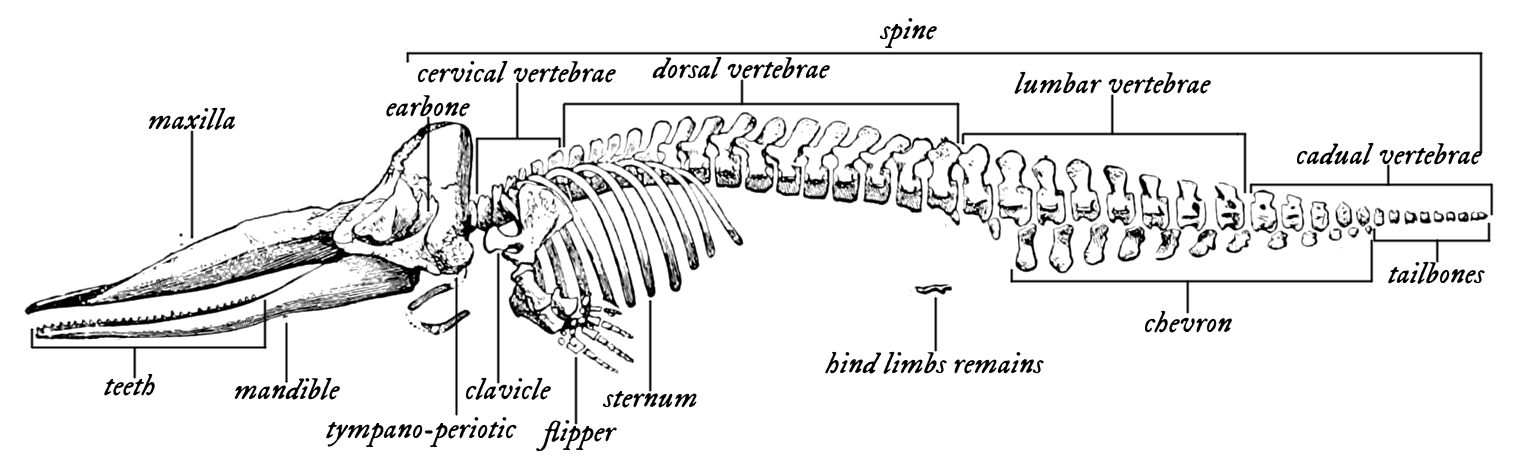
\includegraphics[width=0.99\textwidth]{01yuadrem/img/23sperm_whale_skeleton.png}
    \end{DndTable}
\end{table*}

\subsubsection{Wordbinding\\ \small{Dremshamad}}
Well known is the obsession of the many houses of Palegna with words, names, and languages, and evidence of this is wordbinding.
Wordbinding, or Dremshamad in dust tongue, is the art of giving strength to words so that, no matter the medium, their mere utterance conveys an tangible effect in the world.
Its spells are many and varied, like saving effects in scrolls or books to be invoked later, binding the will of creatures by using their true names, and speaking command words that can't be disobeyed by any mean.

Perhaps the most meaningful product of wordbinding are reflexive contracts.
These agreements bind through the strength of words alone, enforcing their terms upon the signing parties by tying harsh effects to the rights and duties specified.
Always produced in triplicate with each requiring three signatures per party, reflexive contracts are practically unvoidable, thus regarded as the perfect mean to ensure cooperation between beings, houses, or even entire nations.

% Crafting a document with words of power:
% * List of effects that can be produced (more are unlocked as expertise increases)
% * Interaction with words that produce such effect (spoken out loud, whispered, listened to, read)

% All contracts must have a clause that can void the contract by design. Most usually it is being burned by the fire of a wyrm, since this act is neigh impossible without dying.

\subsubsection{Windherding\\ \small{Dentrala}}
Perilous are the winds from the southern ocean, relentlessly tearing apart any ship that dares sail it's turbulent waters.
Many forget that the many tribes from the Qul archipelago had to deal with these strong winds and storms in their daily lives.
To face this, they slowly developed a complex system of sympathetic magic.

By standing atop large poles within eyesight of each other, ird witches from the dentralin tribe managed to stop the wind simply by holding their breath.
This practice gave rise to a wide array of wind-based spells that the tribe wise to use to their advantage during the tunsal wars, and eventually led to the establishing of Jenkash.

\subsubsection{Sigaldry\\ \small{Guen Tsue}}
Unlike other languages, the naenk tongue is deeply rooted in nature itself, and can be used to even directly talk to it, with seedspeech being the clear example.
This quality of the language led to Gannag's shamans to develop a writing system that can evoke effects when interacted with, called shinerunes.

The tsaneks of Gannag use this method to create self-triggering traps, which are set about villages to catch prey and ward off would-be invaders.
Apart from this, intricate shinerunes are used to many different effects, such as a silent bell alerting of the presence of a stranger in a dwelling, a self-heating plate to boil water in, or clothes that spontaneously heat up as a reaction to bad weather.
Truly, the capabilities of shinerunes are only limited by the creativity and skill of their author.

\begin{table*}[t]%
    \begin{DndTable}[width=\linewidth, header=\centering Knaenese Alphabet]{X}
        \centering
        
\includegraphics[width=0.99\textwidth]{01yuadrem/img/23knaenese_sample.png}
    \end{DndTable}
\end{table*}

\subsubsection{Psionics} % NOTE. I don't like the name but it's not that bad I guess.
Perhaps the strangest part of the zaloths is the fact that they do not speak through a mouth, but directly into other beings' minds.
This ability is only made possible by the special nature of the zaloths themselves, and is very rarely seen in the other kins, in peculiar gifted individuals.
Not limited to telepathy however, the art developed into a plethora of mind-based abilities known as psionics.

Psionics are fueled by one's own mind without external sources of energy, meaning that the art exerts a great effort from the author.
The zaloths have elaborated varied psionic effects to date, expanding their original telepathy to more tangible effects, like clairvoyance, telepathy, and many mind-altering effects.

\subsubsection{Similarity Sympathy}
% Blink (quantum teleport): Cantrip to teleport, only usable if being perceived by no sentient being when moving to an area not perceived by any sentient being. Hard to use in most cases yet extremely powerful in certain scenarios. (Mechanically it's a cantrip but using it is actually tiring, so it can't really be used as a reliable method of transportation).
% The best thaumaturges are blind FUCK YES!!

No one can deny that Yuadrem completely changed after the schism.
The ash storm ravaged the land and caused the 9 year famine, tens of thousands of strange creatures poured in, and new, alien kins settled into the land.
For better or for worse, the event transformed the fabric of reality.
Soon after the schism the witches and shamans of the early world started to experiment with a new and strange form of magic: the Similarity Link.

This link is a strange form of sorcery which seems to follow different rules than the other schools.
It affects directly the physical properties of objects and creatures, like making rocks weight as little as feathers, or changing the size of other creatures.
Perhaps the strangest part of this is that it seems to behave differently depending on if it's being perceived or not.%, and thaumaturges take advantage of this by covering their eyes when casting certain spells.

\subsubsection{Tidal Manipulation\\ \small{Rashid}} % !!
Rashid involves manipulating the tides in the air or in others to attain one's goals.
Originally taught by the sole survivor of the Rashiist school of thought, it ranges from simple charms and illusions to potent spells with effects that vary depending on the caster's or target's tidal alignment.

Every Rashid user knows that they must exercise their magic in secrecy, since the practice is severely punished due to Rashiism's dark history.
The most experienced in the art however know that the one they truly have to fear is the Sorrow.
The Sorrow is the being that destroyed the Rashiist school of thought, leaving the pale blemish as a warning to any who dares follow their teachings.

\subsubsection{Fleshshaping\\ \small{Cthai'khas}} % !!
Recently reborn in the breathing city of Cabb Goem-Rlamesh is the almost lost art of Ukarilth: fleshshaping.
An everyday act of the tall kin, fleshshaping is a kind of magic that involves transfiguring the flesh of the caster or of others nearby, be them alive or dead.

While most fleshshapers remain in their putrid island, some have started to show up in the eastern parts of Yuadrem, and the art is slowly being spread by concealed mages.
A strange attribute of fleshshaping that sets it apart from the other schools is that its effect vary depending on the species of the caster.
For example, while a gat can mold its flesh to temporarily use its bones as weapons, a naenk can grow roots into the floor to catch prey, and a quies can reinforce its wooden exterior in preparation for an attack.


% !TEX root = ../main.tex
\begin{figure}[H]
    \centering 
\includegraphics{01yuadrem/img/30history_i.png}
\end{figure}

\section{History} \label{sec::history}
% History is known in detail thanks to the dutiful oths that recorded it under Tol's guidance.
% TODO: Capitalise all the location names, like Arctic Archipelago, Sylvan Canyon, etc.
% TODO: Take a look at the whole cultures and Yuadrem pages and fix years and nation names!

\subsection*{Ancient History}
\subparagraph{682 BS --- First Communion} In the middle of the dead sea, the et E'ukarilth merges with a deceased higher one embryo.
This transforms the tall one into an insane visage of their former self.
The church of E'ukarilth is later founded to attempt communication with the et.

\subparagraph{592 BS --- Birth of Gats} The search for the Lung of Ur begins, an artifact of great value to the tall kin.
The indigo school of the et Thul-yharch creates the hardy gats, believing the relic is below the surface.

\subparagraph{547 BS --- Birth of Irds} With underground search proving unsuccessful, the red school of Zyl'rech births the mobile irds.
Taking to the skies, they survey land and ocean, hoping to find clues of Lung's location.

\subparagraph{523 BS --- Birth of Marsets} The gold school of Tosh-drieln produces the arboreal marsets.
They explore the thick and dark jungles of Yuadrem with ease.

\subparagraph{451 BS --- Birth of Oths} Under mysterious circumstances, oths are created by the et Tol.
Before disappearing, the tall one teaches them writing, and they begin recording history and compiling the findings of the ets and their progeny with great care and detail.

\subparagraph{397 BS --- Ctereth's Workshop} To cope with the uncontrolled population growth of the new kins, the et Ctereth digs a deep cavern in the middle of the dead sea.
Inside it, the tall one builds a workshop and tirelessly crafts qualar to gift the newborns sentience.

\subsection*{Nadir}
\subparagraph{217 BS --- The Rise of the Spire} The tall kin, apparently done with their search, create the spire at the place where E'ukarilth found the higher one.
They build the stone city of Jan'krug atop the mountain.
The progeny kins, now left alone, are forbidden from accessing the dead sea and, incapable of producing qualar, are forced to fight among themselves.

\subparagraph{209 BS --- First Lost Ones} The first plains gats and chu'ash oths are born, separated from their kins by their lack of qualar.
% While ird and marset lost ones also exist, the lack of a qualars doesn't affect these kins as much as their siblings, perhaps due to their wilder nature.

\subparagraph{179 BS --- First Gat City-states} The gats, always fighting adversity, establish the three city-states of Fiele, Avshen, and Alagyaz.
With careful birth control techniques, they manage to maintain a stable population.

\subparagraph{144 BS --- First Siege} A group of three irds known as ``the feathered sunrise'' infiltrates the dead sea and steal tens of thousands of qualar from Ctereth.
The nations of Krudzal, Harual, and Hulnar are later established by their descendants.

\begin{figure}[H]
    \centering 
\includegraphics{01yuadrem/img/30history_ii.png}
\end{figure}

\subparagraph{92 BS --- Naenks \& Tsaneks Discovery} Trying to find a home, a group of stray marsets known as the Ovovians, stumble upon the naenks and tsaneks of Drejeck.
These two are inexplicable kins born from mold and fungi respectively.

\subparagraph{51 BS --- First Artificial Qualars} The gat Jirar the bonecarver creates a technique to craft rough qualars imitations.
By passing the practice to the gat's disciples, Jirar unshackles the population number of the kins, and boosts Alagyaz's economy to unprecedented levels.
% To date, only gat master bonecarvers have managed to use the technique. One bonecarver's qualar count usually doesn't go above the thousands, but as populations grow so does the need for qualar.

\subsection*{Great Famine}
\subparagraph{0 --- The Schism} The tall kin's folly causes the schism.
The spire, now revealed to be a dormant volcano, catastrophically erupts.
The event destroys Jan'krug and most of the ets.
The spewed ash blocks off sunlight for four decades, starting the age known as the great famine.

The explosion causes a portal known as the sizzling gate to be opened in a cave inside of the spire.
This door leads to the outer lands, a strange and primal plane that exists outside of Yuadrem.
From the portal spew forth the foreigner kins: the adventurous tortles, the violent grungs, and the ingenious umans, along with the blueblood beasts.

\subparagraph{1 AS --- Second Siege} The foreigner's horde, a great army of tortles, grungs, and umans, siege Ctereth's workshop.
They're successful, and the great number of qualar stolen is used to start their own settlements in Yuadrem.

\subparagraph{4 AS --- Zaloths Discovery} The zaloths, a kin made of fire, ash, thunder, and hail, walk down from the ruins of Jan'krug.
They freely roam Yuadrem, following a nomadic lifestyle that keeps most away from civilized society.

\subsection*{Age of Heroes}
\subparagraph{38 AS --- End of the Great Famine} Satisfied with a death toll in the tens of millions, the ash clouds from the spire disperse, finally ending the great famine.

\subparagraph{57 AS --- Quies Discovery} A group of gat voyagers from Avshen rise up to Jan'krug, finding the city ruined beyond repair, covered by solidified lava.
However, what they do find beneath the ruins are the quies, a new kin.
Quies are the last kin created by the ets, and are brought back to Avshen.
They easily integrate into gat society, despite their physical differences.

\subparagraph{71 AS --- Start of the Eternal War} The newly born kingdom of Krudzal in the north begins a war against the stone giants of the northern territories.
The war rages to this day, with little obtained by the thul'kraka irds.

\subparagraph{99 AS --- Jenkash's Separation} A blossoming nation of qulbaba irds is split into forty-five separate tribes by ideological differences.

\begin{figure}[H]
    \centering 
\includegraphics{01yuadrem/img/30history_iii.png}
\end{figure}

The tribes that will eventually become Jenkash are bound to constant conflict, unable to establish a unified government for more than a hundred years.

\subparagraph{102 AS --- Third Siege} Inspired by their siblings lost three centuries ago, the army of healing is formed.
Mainly composed of gats and oths, they successfully invade Ctereth's dwellings, then personally bringing the stolen qualar to the bughna gats and the chu'ash oths, re-integrating them into civilized society.

\subparagraph{141 AS --- Birth of Isken} Among the dark forests of the Chirping Wilds, the grung empire of Isken is formed.
Initially secretive, they will soon become one of the most fearsome forces in Yuadrem.

\subparagraph{143 AS --- Babaian Genocide} The grungs of Isken easily crush the marset nation of Baba, systematically killing the marsets until very few are left.

\subparagraph{144 AS --- First Isken-Harual War} Ever hungry for power and land, the Iskean empire attacks the Harualish tribes of the Chirping Wilds.
This is the start of a long sequence of slow and bloody wars that will last for more than two centuries.

\subparagraph{174 AS --- Discovery of the Tides} The oths from the temple of Ignelli, led by Hashim, unearth the phenomenon of the tides, learning of its influence on the kins of Yuadrem.
The discovery revolutionizes the way the kins perceive their own feelings and motivations, and leads to them questioning the nature of sentience itself.

\subparagraph{189 AS --- Fourth Siege} To cope with their ever-growing populations, a temporary alliance is formed between the dratl ird houses of the west and the grung empire of the east.
Their union leads to the fourth and final successful siege of Ctereth, enabling a great growth for the Hulnar and Iskean empires.

\subsection*{Age of Nations}
\subparagraph{195 AS --- Founding of the Seven Kingdoms of the Sea} Ever-growing in numbers, the gat city-states coasting the whaler's sea coalesce into nations, each under its own king.
With all the events happening in one year, the formation of the seven kingdoms of the sea initiate an age of prosperity for the horned and retainer kins.

\subparagraph{201 AS --- Invention of Metal Ships} Edren, a thul'kraka ird from Krudzal, designs and invents the first ironclad ship.
The design, named after the ird's son, Durkin, boosts Krudzal's trading capabilities and kick-starts a great colonization campaign.

\subparagraph{212 AS --- Birth of the Dead Sea Clans} Imitating their neighbors to the north, many uman, dratl ird, and plains gat clans are established in the dead sea.

% These clans however are very different from the civilized kingdoms of the north.
% Warlords are elected by strength, and their territories are as shifting as the erratic sandstorms.

\begin{figure}[H]
    \centering 
\includegraphics{01yuadrem/img/30history_iv.png}
\end{figure}

\subparagraph{229 AS --- Formation of the Jenkashian Empire} Driven by inner conflict, the irds of the qul archipelago exhaust their natural resources.
This forces them to prematurely end their quarrels, and begin invading and pillaging the surrounding territories.

\subparagraph{231 AS --- Ededian Genocide} The Springwater island is almost completely overtaken by Jenkash, decimating the marset population and forcing most into exile.

\subparagraph{247 AS --- Tidal Sway} Hailing from Ignelli, the oth Narr from the Rashiist school of thought performs an uncanny ritual to harness the power of the tides.
This accidentally triggers the tidal sway.

The oth summons the Sorrow into Yuadrem, ending the life of most Rashiists and ravaging the wildlands entirely, blocking access by land to the southern regions of Yuadrem.

\subparagraph{272 AS --- Fifth Siege} The Iskean grungs, banned from buying artificial qualar from Khedrat, attempt a new siege upon Ctereth's workshop.
This time however they fail, stopped by an unsuspected force: the newly formed dead sea clan of Dzarog.
Dzarog is a clan of umans and gats that live in dens around the spire, and protect Ctereth's caverns for yet unknown reasons.

\subparagraph{281 AS --- Creation of Geomancy} The ird nation of Hairuus, protected from Isken by the splitting mountain range, develop the art of geomancy.
As a test of their mastery of it, they elevate an island at the middle of the shield lake, where their capital, the Nest, is built.

\subparagraph{304 AS --- Invention of Gunpowder} Hailing from the young nation of Sulia, the oth Karmin discovers gunpowder.
With this new firepower, many engineers from Sulia design and build varied weapons, like fire spears, hand-cannons, and muskets.
These new weapons give them a proper combat advantage, allowing them to defend themselves from the savage nomadic tribes of the blank plains, and slowly expand their territories to the east.

\subparagraph{331 AS --- Creation of Windherding} The uncommonly peaceful irds from the Dentrala tribe in Jenkash develop the art of windherding.
The other tribes quickly adapt this art for combat, leading to the Drejeck wars against the naenks of Gannag and the Dratl'fal wars against the declining empire of Hulnar.

\subparagraph{340 AS --- Siszgoel's Independence} Siszgoel, a long-standing colony of Krudzal, declares independence.
The nation of Kaldrathal is born, under the rule of the warrior queen Ialul.
The natural deposits of nitrate in the country's island of residence, Krejek, boosts a powerful gunpowder industry, quickly matching that of Sulia.

\begin{figure}[H]
    \centering 
\includegraphics{01yuadrem/img/30history_v.png}
\end{figure}

\subparagraph{354 AS --- Birth of Ribinhep} Umans, a kin commonly hunted an enslaved, manage to establish permanent settlement in the isle of rust.
Naming themselves Ribinhep, they start conquering the northern fjords using their unique mercury weapons, fighting under the rule of the frostburn king Kuin.

\subparagraph{389 AS --- End of the Isken-Harual Wars} After 248 years, the Isken-Harual wars end, with Isken crushing almost all of the ird tribes.
The grung empire quickly proceeds to attack the Byurev nation, attempting to conquer territories up north.
They are however stopped by the gats, prepared for such an invasion decades ago.

\subparagraph{411 AS --- Vanishing of Hairuus} The lake-based country of Hairuus suddenly vanishes, soon after elevating new land for their growing capital.
Rumors that the lake is haunted begin spreading, and nations avoid claiming the empty territories and abandoned cities for fear of this mysterious curse.

\subparagraph{440 AS --- Gannag Invasion} Seeing that the Jenkashian forces are focused on conquering the mainland, the armies of Gannag suddenly invades the qul archipelago under the command of Kutsa the sharp.
In few weeks they manage to conquer half of Jenkash's homeland, taking prisoner irds as sacrifices to use as birth corpses.

\subparagraph{461 AS --- Kaldrathal's Conquest} Most of the islands of the arctic archipelago are claimed by Kaldrathal, who establishes a new form of government that tries to represent the taken territories.

\subparagraph{498 AS --- Invention of Blast Weapons} Reut, an engineer from Drer, invents a new use of Sulia's gunpowder: Blast weapons.
Used for close-quarters combat, blast weapons aim to both surprise and immolate the enemy.
Among the most famous examples are the flame vent, the firecrackers and the flaming pole-arms.

\subparagraph{533 AS --- Creation of Wordbinding} In collaboration, the many oth houses of Palegna create the art of wordbinding.
The technique quickly gains traction, as it adds a method for trustless trade between peoples and nations.

% \subparagraph{553 AS --- Na'ane's Founding} A large circle of tsaneks led by Tsehant, tired of their class-based society, made a pilgrimage to the fog gorge.
% They establish in it, and form the independent nation of Na'ane.

\subparagraph{577 AS --- Establishment of Tanethism} The king of Khedrat, Grigor the Old, establishes the recently born Tanethism as the official religion of the nation.
The other kingdoms of the sea follow soon after, and Tanethism is quickly adopted by most gats.
% Here is when bonereading becomes accepted in the seven kingdoms.

\subparagraph{589 AS --- Appearance of Fo} Strange, twisted creatures start attacking any village coasting the shield lake, causing havoc.
Fo, the kinless inhabitant of the nest is quickly blamed for the creation of this creatures, but all attempts to reach the being have failed.

\begin{figure}[H]
    \centering 
\includegraphics{01yuadrem/img/30history_vi.png}
\end{figure}

\subsection*{Golden Age}
\subparagraph{591 AS --- Hulnar's Demise} The strong alliance between the nations of Khedrat and Sulia defeats Hulnar in the Sylvan wars, allowing both nations to occupy a segment of the Ichor mountains and the entirety of the Sylvan canyon.
This act helps mitigate the pirates' presence in the Whaler's Sea, kick-starting an era of peace and trade for the coastal nations.

\subparagraph{599 AS --- Invention of Steel Firearms} The inventive Kaldrathian engineer Seja combines Krudzal's quench-hardened steel with her new refined gunpowder.
The explosive mix leads to the development of fierce steel-based weapons, including long-range cannons, wheel-lock pistols and sophisticated rifles.

\subparagraph{607 AS --- Invention of the Steam Engine} Away from the economic center of Yuadrem, the Na'anian tsanek Nugut invents the steam engine.
Originally used simply to drain the Na'anian coal mines, the tsaneks were quick to notice its potential and found hundreds of applications for the engine over time.

\subparagraph{621 AS --- The Penance} A surreptitious ritual known only as ``The Penance'' is carried by the citizens of Dzarog.
From the top of the spire, they summon a horrible being known as Cabb Goem-Rlamesh into Yuadrem.
The colossal amalgamate of flesh slowly drags itself towards the east, ferociously protected by the Dzarogian armies.

\subparagraph{628 AS --- Krudzal's First Victory} Using modified Kaldrathal cannons, Krudzal finally manages to kill a stone giant, claiming their first victory in the Eternal War.
% The event strikes fear on the giants, and Krudzal manages to claim their first territories in the mainland.

\subparagraph{635 AS --- Dissolution of Hulnar} Heirless, the king Sul'rech of Hulnar suddenly dies at a young age.
The dwindling kingdom is split into smaller houses, weak ghosts of Hulnar's old glory.

\subparagraph{655 AS --- Cabb Goem-Rlamesh's Launching} The harrowing immensity, Cabb Goem-Rlamesh, reaches the Burnt Ocean and settles some kilometers off the coast of the dry savanna.
% It becomes known as the breathing city.
% All expeditions to the island have ended poorly.

\subparagraph{659 AS --- Separation of Khedrat} The newly-conquered westernmost territories of Khedrat quickly become tired of monarchy, and peacefully claim independence.
Abandoning old traditions, the new countries of Viphogher and Dnomit embrace democracy: a new, king-less form of government.

\subparagraph{671 AS --- Jenkash's Reclaiming} Forced by Gannag to halt their conquest, the Jenkashian empire focused entirely on re-taking the qul archipelago.
Savage battles are fought, and to date they've managed to reclaim most of their lost homeland.

\subparagraph{672 AS --- Present Day}
\newpage

